% Template for Cogsci submission with R Markdown

% Stuff changed from original Markdown PLOS Template
\documentclass[10pt, letterpaper]{article}

\usepackage{cogsci}
\usepackage{pslatex}
\usepackage{float}
\usepackage{caption}

% amsmath package, useful for mathematical formulas
\usepackage{amsmath}

% amssymb package, useful for mathematical symbols
\usepackage{amssymb}

% hyperref package, useful for hyperlinks
\usepackage{hyperref}

% graphicx package, useful for including eps and pdf graphics
% include graphics with the command \includegraphics
\usepackage{graphicx}

% Sweave(-like)
\usepackage{fancyvrb}
\DefineVerbatimEnvironment{Sinput}{Verbatim}{fontshape=sl}
\DefineVerbatimEnvironment{Soutput}{Verbatim}{}
\DefineVerbatimEnvironment{Scode}{Verbatim}{fontshape=sl}
\newenvironment{Schunk}{}{}
\DefineVerbatimEnvironment{Code}{Verbatim}{}
\DefineVerbatimEnvironment{CodeInput}{Verbatim}{fontshape=sl}
\DefineVerbatimEnvironment{CodeOutput}{Verbatim}{}
\newenvironment{CodeChunk}{}{}

% cite package, to clean up citations in the main text. Do not remove.
\usepackage{apacite}

% KM added 1/4/18 to allow control of blind submission


\usepackage{color}

% Use doublespacing - comment out for single spacing
%\usepackage{setspace}
%\doublespacing


% % Text layout
% \topmargin 0.0cm
% \oddsidemargin 0.5cm
% \evensidemargin 0.5cm
% \textwidth 16cm
% \textheight 21cm

\title{Developmental shifts in children's use of register-specific
words}

\usepackage{booktabs}
\usepackage{longtable}
\usepackage{array}
\usepackage{multirow}
\usepackage{wrapfig}
\usepackage{float}
\usepackage{colortbl}
\usepackage{pdflscape}
\usepackage{tabu}
\usepackage{threeparttable}
\usepackage{threeparttablex}
\usepackage[normalem]{ulem}
\usepackage{makecell}
\usepackage{xcolor}

\author{{\large \bf Kennedy Casey} \\ University of Chicago \\ \texttt{kbcasey@uchicago.edu} \And {\large \bf Marisa Casillas} \\ University of Chicago \\ \texttt{mcasillas@uchicago.edu}}

\newlength{\cslhangindent}
\setlength{\cslhangindent}{1.5em}
\newenvironment{CSLReferences}%
  {}%
  {\par}

\begin{document}

\maketitle

\begin{abstract}
Child-directed language (CDL) features words such as \emph{doggy},
\emph{night-night}, and \emph{tummy} that are rarely used in
adult-directed language (ADL). Characterisitcs of CDL word forms, such
as diminutivization and reduplication, explain why they may be learned
and produced earlier by children. However, it is not yet clear how or
when children switch to using ADL equivalents---\emph{dog},
\emph{goodnight}, \emph{stomach}. Through analysis of speech transcripts
from CHILDES and the Language Development Project corpus, we show that
children significantly increase their production of ADL word forms
across age, with the average CDL-to-ADL transition point at 2.5 years.
Many of the linguistic features that distinguish CDL vs.~ADL registers
(e.g., lexical and syntactic complexity) similarly differentiated the
local speech contexts surrounding CDL vs.~ADL word forms in children's
input. Learners may therefore be able to capitalize on these cues to
support their discovery of register along with context-appropriate
CDL/ADL pair use.

\textbf{Keywords:}
child-directed language; word production; linguistic input; social
register; corpus analysis; developmental change
\end{abstract}

\hypertarget{introduction}{%
\section{Introduction}\label{introduction}}

Across their first few years of life, children come to know hundreds if
not thousands of words (Fenson et al., 1994; Mayor \& Plunkett, 2011).
Word production typically begins around age one, followed by a
vocabulary `explosion' or `spurt' during toddlerhood (Ganger \& Brent,
2004; see also McMurray, 2007), and then continued, measurable increases
in vocabulary size thereafter (Rice \& Hoffman, 2015). Here, we
investigate one dimension of this dramatic developmental change: the
appearance and use of words from distinct registers.

Vocabulary first gets off the ground, in part, with words that are
specifically tailored to young learners (e.g., \emph{tummy}, Ferguson,
1964). Hallmark features of child-directed language (CDL), such as
iconicity (Laing, Vihman, \& Keren-Portnoy, 2017), diminutivization
(Kempe, Brooks, \& Gillis, 2005), and reduplication (Ota,
Davies-Jenkins, \& Skarabela, 2018) may support early word learning.
These effects are in addition to the cross-cutting influence of a word's
frequency, concreteness, length, and association with infancy on early
learnability (e.g., \emph{bottle} and \emph{bib}: Braginsky, Yurovsky,
Marchman, \& Frank, 2019; Frank, Braginsky, Yurovsky, \& Marchman, 2017;
Perry, Perlman, Winter, Massaro, \& Lupyan, 2018).

While CDL-specific words (e.g., \emph{night-night}, \emph{doggy},
\emph{tummy}) are overrepresented in children's early vocabularies, they
are eventually replaced by ADL equivalents (\emph{goodnight},
\emph{dog}, \emph{stomach}). However, these words do not fully
disappear. Instead, they become designated for use in a specific
context---communication with infants and young children (e.g., Sachs \&
Devin, 1976; Shatz \& Gelman, 1973). The addition of a word like
\emph{stomach} to a children's vocabularies may mark their growing
awareness that word choice should be tailored to the current
interactional context (Clark, 1997, e.g., 2018). We do not, at present,
know when children begin to make shifts from CDL to ADL word use or
precisely how such a shift is supported or initiated. Our investigation
starts where this transition is most easily observed, with CDL/ADL word
pairs: (e.g., \emph{doggy/dog}, \emph{night-night/goodnight},
\emph{tummy/stomach}), as opposed to words that become less relevant
with time (e.g., \emph{diaper} and \emph{peekaboo}).

\hypertarget{comprehension-and-production-of-language-varieties}{%
\subsection{Comprehension and production of language
varieties}\label{comprehension-and-production-of-language-varieties}}

Classically, we might expect the appearance of both CDL and ADL labels
for the same referent to be a problem for early word
learning---particularly when the variants have little to no overlap in
phonological form (e.g., \emph{bunny/rabbit} vs.~\emph{doggy/dog}).
Indeed, children often assume that new labels refer to new items rather
than interpreting them as synonyms for words that they already know
(i.e., {``mutual exclusivity''}: Markman \& Wachtel, 1988; see Lewis,
Cristiano, Lake, Kwan, \& Frank, 2020, for a recent meta-analysis). Yet,
children seem to learn multiple CDL/ADL variants without issue.

One potential way to explain children's learning of both labels is to
consider the social context of CDL vs.~ADL use. While labeling an animal
as \emph{doggy} vs.~\emph{dog} may not communicate anything distinct
about the referent itself, the production of one form vs.~the other may
indicate something meaningful about \emph{who} is being addressed or
producing the label. That is, differences in register could serve to
`explain away' the otherwise problematic redundancy of multiple labels
in these pairs (Clark, 1990). Indirect evidence for this idea comes from
findings that the mutual exclusivity effect is modulated by children's
experience with multiple languages (Byers-Heinlein \& Werker, 2009;
Houston-Price, Caloghiris, \& Raviglione, 2010) and the social
conditions under which multiple labels are introduced (e.g., by speakers
of a familiar or unfamiliar race: Weatherhead, Kandhadai, Hall, \&
Werker, 2021). Further, children's speech to younger children (Sachs \&
Devin, 1976; Shatz \& Gelman, 1973) and their awareness of socially
meaningful linguistic variation (Ikeda, Kobayashi, \& Itakura, 2018;
Liberman, Woodward, \& Kinzler, 2017; Soley \& Sebastian-Galles, 2020)
suggests that they recognize the importance of social context for
language use from relatively early on.

We hypothesize that children may contend with CDL/ADL word pairs by
associating the contrasting forms with different modes of use (i.e., by
classifying each form as belonging to a distinct register). To test this
idea, we first need to establish (a) when children begin to shift away
from producing CDL-specific words, and (b) how children may be able to
use bottom-up linguistic input cues to associate lexical variants with
their associated registers (i.e., CDL vs.~ADL).

\hypertarget{current-investigation}{%
\subsection{Current investigation}\label{current-investigation}}

We examine a small but core subset of 15 CDL-specific words in English
(e.g., \emph{doggy}, \emph{night-night}, \emph{tummy}) that are
prevalent in children's early vocabularies but are eventually replaced
by ADL words---\emph{dog}, \emph{goodnight}, \emph{stomach}. In Study 1,
we analyze over 60,000 utterances of spontaneous speech from children up
to seven years of age to establish when ADL forms become more dominant
in children's own productions. That is, when do children switch from
using CDL forms to using ADL forms? Our data suggest that the average
age of `CDL-to-ADL switchover' occurs around 2.5 years.

We then explore the features of children's input that could support this
switch by examining the extent to which CDL and ADL words are used in
distinct linguistic contexts by adults. Further processing of nearly
70,000 non-target-child utterances (primarily from adult caregivers and
addressed to the target child) revealed that CDL and ADL variants
co-occur with reliably different patterns of prosodic, lexical, and
syntactic information---cues that likely help learners associate them
with different modes of use, or emerging representations of register.

Together, these studies push us to consider children's vocabulary
development not as a simple accumulation of words or numeric increase in
vocabulary size but rather a deepening and restructuring of the lexicon
with growing linguistic and social maturity. The words \emph{dog} and
\emph{stomach} do not entirely replace \emph{doggy} and
\emph{tummy}---rather, the contrasting forms become reserved for use
with different addressees.

\hypertarget{study-1-when-do-children-shift-from-cdl-to-adl-forms}{%
\section{Study 1: When do children shift from CDL to ADL
forms?}\label{study-1-when-do-children-shift-from-cdl-to-adl-forms}}

We tracked children's use of 15 CDL/ADL word pairs (Table 1) from early
infancy up to age seven. Since CDL forms rarely appear in ADL, we
predicted that children would shift away from production of these
CDL-specific forms with increasing age. That is, we expected to see
replacement of CDL forms with ADL forms in children's own speech across
time.

\hypertarget{method}{%
\section{Method}\label{method}}

\hypertarget{corpora}{%
\subsection{Corpora}\label{corpora}}

We analyzed 8,251 transcripts in the North American English collection
of the Child Language Data Exchange System (CHILDES) database
(MacWhinney, 2000) for children up to 7 years of age. The included
transcripts were drawn from 52 individual corpora and featured 980
children (age range = 1--84 months, \emph{M} = 33.5 months). To further
gain purchase on our research question with \emph{longitudinal} data, we
also analyzed child production data from the Language Development
Project (LDP) corpus (see Huttenlocher, Waterfall, Vasilyeva, Vevea, \&
Hedges, 2010; Rowe, 2008, for further details regarding participating
families, recording procedures, and transcription). LDP data included
622 transcripts from 59 English-learning children recorded every 4
months for approximately 90 minutes from age 14 to 58 months.

\hypertarget{target-words}{%
\subsection{Target words}\label{target-words}}

Fifteen CDL/ADL word pairs (30 total target words) were selected based
on two criteria: the appearance of at least one form on the
MacArthur-Bates Communicative Development Inventory (CDI, Fenson et al.,
1994), and sufficient frequency of occurrence in CHILDES (at least 100
child-produced tokens and 100 other-produced tokens per form). Pairs
were also selected based on our own subjective judgment that the same
object, animal, routine, or body part could be reasonably labeled with
either form by young children.\footnote{While onomatopoeic words can be
  used in a similar manner to the CDL-specific words in our test set
  (e.g., \emph{choo-choo} serving as a CDL-specific label for
  \emph{train}, or \emph{quack-quack} for \emph{duck}), these iconic
  items were not included because they are primarily used as sound
  effects rather than labels for objects or animals (Skarabela, Pool, \&
  Ota, 2018). The polysemous nature of iconic word usage does not
  provide as clear of a test of replacement of CDL forms with ADL forms
  over time.} Across all transcripts, 64,852 child-produced utterances
contained at least one target word and were included in our analysis.

\begin{table}[!h]

\caption{\label{tab:tab:tab1}CHILDES frequency for 15 CDL/ADL word pairs. Child-produced counts include tokens produced only by the target child.}
\centering
\fontsize{7}{9}\selectfont
\begin{tabu} to \linewidth {>{}l>{\centering}X>{\centering}X>{\centering}X>{\centering}X}
\toprule
\multicolumn{1}{c}{\textbf{ }} & \multicolumn{2}{c}{\textbf{CDL tokens}} & \multicolumn{2}{c}{\textbf{ADL tokens}} \\
\cmidrule(l{3pt}r{3pt}){2-3} \cmidrule(l{3pt}r{3pt}){4-5}
\textbf{Pair} & \textbf{Child} & \textbf{Other} & \textbf{Child} & \textbf{Other}\\
\midrule
\em{doggy/dog} & 2,249 & 2,644 & 3,519 & 5,113\\
\em{kitty/cat} & 1,552 & 3,309 & 2,779 & 4,443\\
\em{tummy/stomach} & 435 & 623 & 112 & 360\\
\em{daddy/dad} & 9,603 & 10,048 & 2,313 & 1,031\\
\em{mommy/mom} & 20,294 & 17,070 & 7,616 & 2,552\\
\em{bunny/rabbit} & 1,237 & 2,597 & 1,060 & 1,397\\
\em{duckie/duck} & 307 & 647 & 1,933 & 3,003\\
\em{blankie/blanket} & 174 & 224 & 825 & 874\\
\em{froggy/frog} & 154 & 434 & 970 & 1,846\\
\em{potty/bathroom} & 511 & 786 & 161 & 270\\
\em{night night/goodnight} & 149 & 153 & 102 & 446\\
\em{dolly/doll} & 745 & 1,054 & 674 & 2,697\\
\em{horsey/horse} & 1,149 & 1,034 & 1,749 & 2,575\\
\em{piggy/pig} & 405 & 1,212 & 1,276 & 2,139\\
\em{birdie/bird} & 399 & 588 & 1,879 & 3,358\\
\bottomrule
\end{tabu}
\end{table}

\hypertarget{results}{%
\section{Results}\label{results}}

We asked when CDL forms are replaced by ADL forms in children's own
speech. Using the \emph{lme4} package (version 1.1.27.1: Bates, Mächler,
Bolker, \& Walker, 2015) in R (version 4.1.0: R Core Team, 2021), we fit
a mixed-effects binomial logistic regression model predicting children's
production of CDL vs.~ADL forms, with target child age (in months,
scaled) as a single fixed effect. Random slopes and intercepts for word
pairs were also included\footnote{glmer(form \(\sim\) age (months,
  scaled) + (1 + age \textbar{} word pair), family = binomial)}. For
each target word token, the form was coded as either 0 (CDL) or 1 (ADL).
Thus, the model captures, for each age, the probability of using ADL
forms over CDL forms.

Children significantly increased their production of ADL forms over age
(\(\beta\) = 0.54, \emph{SE} = 0.11, \emph{t} = 4.92, \emph{p}
\textless{} 0.001). The average CDL-to-ADL transition point (i.e., the
point at which ADL forms were produced \textgreater50\% of the time) was
at approximately 28 months (i.e., around 2.5 years; Figure 1).

The trend of increasing ADL form production was significant for 13 of 15
word pairs, but the exact trajectory of shift varied greatly across
items (Figure 2). In some cases, CDL forms were replaced by ADL forms
early on (e.g., \emph{doggy/dog} and \emph{kitty/cat} around 2 years).
For other pairs, the age of switchover was much later (e.g.,
\emph{tummy/stomach} and \emph{potty/bathroom} around 5 years). Finally,
a clear point of switchover was not observed for some pairs because ADL
forms were already produced \textgreater50\% of the time from the
earliest ages sampled (e.g., \emph{duckie/duck} and
\emph{blankie/blanket}).

\begin{CodeChunk}
\begin{figure}[h]

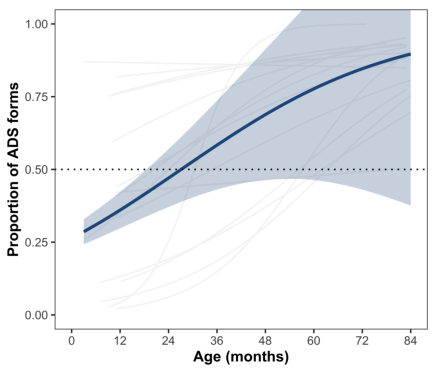
\includegraphics{figs/shift-timing-fig-1} \hfill{}

\caption[Model-predicted increase in production of ADL forms across age, with shaded standard error region]{Model-predicted increase in production of ADL forms across age, with shaded standard error region. Gray lines depict individual word-pair trajectories.}\label{fig:shift-timing-fig}
\end{figure}
\end{CodeChunk}

\begin{CodeChunk}
\begin{figure}[!ht]

{\centering 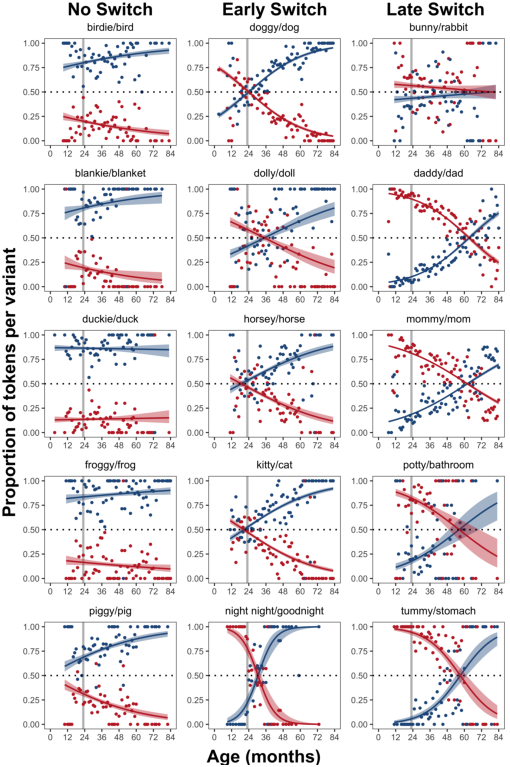
\includegraphics{figs/shift-timing-bypair-fig-1} 

}

\caption[Individual word-pair trajectories for increasing production of ADL forms (blue) and decreasing production of CDL forms (red) with age]{Individual word-pair trajectories for increasing production of ADL forms (blue) and decreasing production of CDL forms (red) with age. Points indicate proportions for each 1-month age bin. Vertical gray lines at 28 months indicate the overall model-predicted CDL-to-ADL transition point across all words.}\label{fig:shift-timing-bypair-fig}
\end{figure}
\end{CodeChunk}

\hypertarget{discussion}{%
\section{Discussion}\label{discussion}}

Analysis of children's own spontaneous speech revealed development
shifts in their production of CDL vs.~ADL forms, with the latter
becoming increasingly more prominent over age. While we found
substantial variation in the exact trajectories of CDL-to-ADL vocabulary
shift for the 15 word pairs, the overall trend towards ADL production
was clear. We take children's shifts away from CDL forms and towards ADL
forms as indirect evidence of their early formation of CDL and ADL as
distinct registers.

\hypertarget{study-2-what-linguisitc-information-in-childrens-input-supports-their-shift-from-cdl-to-adl-forms}{%
\section{Study 2: What linguisitc information in children's input
supports their shift from CDL to ADL
forms?}\label{study-2-what-linguisitc-information-in-childrens-input-supports-their-shift-from-cdl-to-adl-forms}}

We next explored children's input (i.e., other-produced speech), asking
what linguistic information could support their shift from CDL to ADL
forms. We conceptualize our second study as an investigation of the cues
that could help learners associate CDL and ADL words with their
appropriate registers.

CDL, as a register, is differentiated from ADL at multiple linguistic
levels, including prosodic, lexical, and syntactic differentiations
(e.g., Soderstrom, 2007). In English, CDL is associated with higher
overall pitch as well as greater variability in pitch contours (Fernald,
1989; Vosoughi \& Roy, 2012). CDL utterances are often produced more
slowly (Ko \& Soderstrom, 2013; e.g., Vigliocco, Shi, Gu, \& Grzyb,
2020; but see also Martin, Igarashi, Jincho, \& Mazuka, 2016). CDL also
typically includes less lexical diversity (Hills, 2013) and more words
that children already know (Foushee, Griffiths, \& Srinivasan, 2016).
Syntactically, CDL is characterized as less complex than ADL. CDL
utterances are typically shorter (Brent \& Siskind, 2001; Martin,
Igarashi, Jincho, \& Mazuka, 2016) and feature simpler constructions
(Cameron-Faulkner, Lieven, \& Tomasello, 2003).

Here, we tested whether the linguistic features that differentiate CDL
vs.~ADL at the register level also differentiate the local speech
contexts surrounding CDL vs.~ADL forms---even in speech that is
primarily addressed to children from their primary caregivers (i.e.,
language from a single register). In other words, can form be predicted
on the basis of individual utterance-level prosodic, lexical, or
syntactic cues?

We hypothesized that utterances with CDL forms, relative to utterances
with ADL forms, would be associated with (1) higher mean pitch, (2)
greater pitch variability, (3) slower speaking rates, and (4) less
lexical complexity. We also predicted that CDL utterances would contain
(5) fewer rare words, (6) fewer words overall, and (7) fewer verb
phrases. If these linguistic cues reliably differentiate CDL vs.~ADL
word usage contexts, then they could provide a viable source of
information to support children's association between these words and
their corresponding registers.

\begin{CodeChunk}
\begin{figure*}[h]

{\centering 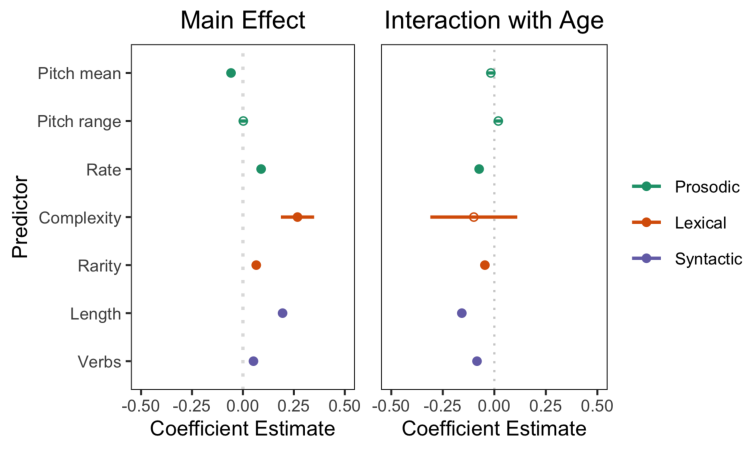
\includegraphics{figs/ling-predictors-fig-1} 

}

\caption[Coefficient estimates for linguistic predictors of form]{Coefficient estimates for linguistic predictors of form. Positive main effects indicate that utterances are more likely to contain ADL forms when they have higher values for that predictor (e.g., faster speech rates). Positive age interactions indicate an increasing effect of the predictor with age. Error bars depict standard errors of the coefficient estimates, and filled circles represent significant effects (\textit{p} $<$ 0.05).}\label{fig:ling-predictors-fig}
\end{figure*}
\end{CodeChunk}

\hypertarget{method-1}{%
\section{Method}\label{method-1}}

\hypertarget{corpora-1}{%
\subsection{Corpora}\label{corpora-1}}

We analyzed 69,709 other-produced utterances (i.e., utterances not
produced by the target child) in the same CHILDES transcripts from Study
1. The majority of utterances were produced by children's primary
caregivers (\emph{n} = 58,071, or 83.3\%).

\hypertarget{linguistic-input-predictors}{%
\subsection{Linguistic input
predictors}\label{linguistic-input-predictors}}

All input analyses were conducted over individual utterances containing
at least one of the 30 target words from Study 1. We quantified
prosodic, lexical, and syntactic information to describe each utterance.

\hypertarget{prosodic-level}{%
\subsubsection{Prosodic level}\label{prosodic-level}}

We measured three types of prosodic information: \textbf{mean pitch}
(Hz), \textbf{pitch range} (Hz), and \textbf{speech rate} (words per
second). These measures were calculated over all timestamped utterances
in CHILDES (42.3\% of other-produced utterances). Utterances shorter
than 58 ms were excluded from analysis.\^{}{[}This lower bound was set
by identifying the the shortest possible duration of an utterance
containing at least one word in four manually annotated North American
English corpora (see Bergelson et al., 2019 for details) Pitch
information was extracted using Praat software (Boersma \& Weenink,
2016).

\hypertarget{lexical-level}{%
\subsubsection{Lexical level}\label{lexical-level}}

We measured two types of lexical information: complexity and rarity.
\textbf{Lexical complexity} was defined as the negative log proportion
of known words in each utterance (consistent with Foushee, Griffiths, \&
Srinivasan, 2016; Kidd, Piantadosi, \& Aslin, 2012). A word was
considered `known' if the age of acquisition (AoA) estimate (Fenson et
al., 1994; Frank, Braginsky, Yurovsky, \& Marchman, 2017) was less than
or equal to the age of the target child when they heard the utterance.
Utterances with proportionally fewer known words are considered more
lexically complex. \textbf{Lexical rarity} was determined based on
overall frequency in CHILDES. For all words with at least 10
tokens\footnote{Manual checks revealed that many of the lowest-frequency
  words in CHILDES included idiosyncratic or erroneous transcriptions,
  so we excluded words with fewer than 10 tokens from our estimates of
  lexical rarity to reduce noise in this measure.}, we calculated a
rarity score as the negative log proportion of other-produced tokens in
CHILDES (i.e., number of tokens for a given word divided sum of all
tokens of all words in the full corpus). We then averaged the rarity
scores for all individual words in a given target utterance. Utterances
with more low-frequency words are considered more lexically rare.

\hypertarget{syntactic-level}{%
\subsubsection{Syntactic level}\label{syntactic-level}}

Syntactic measures included both the utterance \textbf{length} (in
words) and \textbf{number of verb phrases}. The number of words per
utterance was automatically extracted using the \emph{childesr} package
(Braginsky, Sanchez, \& Yurovsky, 2021). The number of verb phrases per
utterance was determined using \emph{spaCy3}, an automatic syntactic
parser (Honnibal, Montani, Van Landeghem, \& Boyd, 2020).

\hypertarget{results-1}{%
\section{Results}\label{results-1}}

We ran individual mixed-effects binomial logistic regression models of
ADL or CDL word form use for each of seven linguistic input predictors.
Models included fixed effects of linguistic predictor (scaled), target
child age (in months, scaled), and their interaction as well as random
intercepts for individual word pairs and speakers\footnote{Model
  strucutre: glmer(form \textasciitilde{} linguistic predictor (numeric,
  scaled) * age (months, scaled) + (1 \textbar{} word pair) + (1
  \textbar{} speaker)}. For each target word token, the form was coded
as CDL (0) or ADL (1), so coefficient estimates provide a measure of the
strength of association between a predictor and ADL form. All main
effects of linguistic predictors and interactions with age are shown in
Figure 3.

At the prosodic level, we found significant effects for two of the three
input predictors tested. Utterance-level \textbf{pitch range} was not
predictive of form (\(\beta\) = 0.002, \emph{SE} = 0.02, \emph{t} =
0.10, \emph{p} = 0.919) and did not significantly interact with age
(\(\beta\) = 0.02, \emph{SE} = 0.02, \emph{t} = 1.11, \emph{p} = 0.268).
However, utterance-level \textbf{mean pitch} was a negative predictor of
ADL form (\(\beta\) = -0.058, \emph{SE} = 0.02, \emph{t} = -3.02,
\emph{p} = 0.003). That is, utterances with higher overall mean pitch
were more likely to contain CDL forms, with no significant interaction
with age (\(\beta\) = -0.02, \emph{SE} = 0.02, \emph{t} = -0.96,
\emph{p} = 0.337). \textbf{Speech rate} (i.e., words produced per
second) was a positive predictor of ADL form (\(\beta\) = 0.09,
\emph{SE} = 0.02, \emph{t} = 4.86, \emph{p} \textless{} 0.001).
Utterances spoken more quickly were more likely to contain ADL forms.
This input predictor also negatively interacted with age (\(\beta\) =
-0.07, \emph{SE} = 0.02, \emph{t} = -3.96, \emph{p} \textless{} 0.001),
indicating a decreasing strength in predictive power across
developmental time.

At the lexical level, we found significant effects for both input
predictors tested. Utterances with higher levels of \textbf{lexical
complexity} (\(\beta\) = 0.27, \emph{SE} = 0.08, \emph{t} = 3.28,
\emph{p} = 0.001) and \textbf{lexical rarity} (\(\beta\) = 0.07,
\emph{SE} = 0.01, \emph{t} = 5.73, \emph{p} \textless{} 0.001) were more
likely to contain ADL forms. Lexical complexity did not interact with
age (\(\beta\) = -0.10, \emph{SE} = 0.21, \emph{t} = -0.47, \emph{p} =
0.637); whereas, lexical rarity negatively interacted with age such that
there was a decreasing effect of this predictor over time (\(\beta\) =
-0.05, \emph{SE} = 0.01, \emph{t} = -3.95, \emph{p} \textless{} 0.001).

At the syntactic level, we found significant effects of
\textbf{utterance length} and \textbf{number of verb phrases}.
Utterances with more words (\(\beta\) = 0.19, \emph{SE} = 0.01, \emph{t}
= 16.30, \emph{p} \textless{} 0.001) and more verb phrases (\(\beta\) =
0.05, \emph{SE} = 0.01, \emph{t} = 4.44, \emph{p} \textless{} 0.001)
were more likely to contain ADL forms. Moreover, both linguistic
predictors negatively interacted with age (Length: \(\beta\) = -0.16,
\emph{SE} = 0.01, \emph{t} = -14.61, \emph{p} \textless{} 0.001; Verbs:
\(\beta\) = -0.08, \emph{SE} = 0.01, \emph{t} = -7.70, \emph{p}
\textless{} 0.001), suggesting that the strength of these predictors
decreases across developmental time.

\hypertarget{discussion-1}{%
\section{Discussion}\label{discussion-1}}

Analyses of children's input revealed reliable differences in the
patterns of linguistic information surrounding CDL vs.~ADL forms. Many
of the prosodic, lexical, and syntactic features that broadly
differentiate CDL vs.~ADL registers similarly partitioned utterances
containing CDL vs.~ADL forms. Notably, these differences in local speech
context emerged even in language that was primarily addressed to
children from their primary caregivers (i.e., language likely from a
single register---CDL).

While we do not yet know if these linguistic cues are actually exploited
by learners, this study identifies which patterns appear learnable in
principle. More broadly, this work provides support for the possibility
that associations with CDL vs.~ADL registers are helping learners grasp
the differences in the context of CDL vs.~ADL form use and gradually
transition away from use of more contextually-constrained CDL-specific
words. A next step is to experimentally test how well children across
this age range perceive words as CDL or ADL relevant given the
surrounding linguistic context.

\hypertarget{general-discussion}{%
\section{General Discussion}\label{general-discussion}}

In the current work, we establish that children shift away from
production of CDL-specific words over age. As predicted, these
child-centric words are `replaced' by ADL equivalents---at least until
they again become relevant when talking to younger children. Further, we
identify patterns in children's linguistic input that could support
their discovery of associations between CDL/ADL words and their typical
modes of use (i.e., incipient representations of register).

\hypertarget{more-than-vocabulary-size-understanding-words-and-using-them-in-context}{%
\subsection{More than vocabulary size: Understanding words and using
them in
context}\label{more-than-vocabulary-size-understanding-words-and-using-them-in-context}}

By analyzing spontaneous language production in the present study, we
find variation in form that is often overlooked but may be crucial for
understanding how vocabularies develop. Popular caregiver-reported
(Fenson et al., 1994) and researcher-administered (Dunn \& Dunn, 1965)
vocabulary measures typically ask for a binary indication of whether a
child `knows' a word. For good reason, these surveys and tests often
gloss over variations in form. This standardization helps with
generalizing over many idiosyncracies, allowing for large-scale, even
cross-linguistic comparisons (e.g., Frank, Braginsky, Yurovsky, \&
Marchman, 2017, 2021). At the same time, glossing over variations in
form presents a missed opportunity to investigate more nuanced aspects
of vocabulary development. The present findings on the transition
between CDL and ADL forms help demonstrate that vocabulary development
taps into other major aspects of children's language learning, including
their socialization as users of the language in their community.

\hypertarget{developing-linguistic-and-social-knowledge-in-tandem}{%
\subsection{Developing linguistic and social knowledge in
tandem}\label{developing-linguistic-and-social-knowledge-in-tandem}}

Children's linguistic knowledge builds around and together with their
social knowledge. The lexical variants of CDL vs.~ADL registers are just
one example of socially meaningful linguistic variation. Variation also
appears across languages, dialects, accents, and other types of
registers (e.g., pedagogical, narrative, etc.). We focus here on
multiple labels for the same referent, but learners also face the
inverse problem: one label for different referents (e.g., Casey, Potter,
Lew-Williams, \& Wojcik, 2021; Meylan, Mankewitz, Floyd, Rabagliati, \&
Srinivasan, 2021). We see these puzzles of word learning as
interrelated; learning is happening at multiple levels---not just the
words themselves, but strong associations between words and their
surrounding contexts (linguistic, social, etc.). Considering the
interaction between these different factors can help us reason about
learning mechanisms and children's representations---again not just of
words but related social information too.

\hypertarget{references}{%
\section{References}\label{references}}

\setlength{\parindent}{-0.1in} 
\setlength{\leftskip}{0.125in}

\noindent

\hypertarget{refs}{}
\begin{CSLReferences}{1}{0}
\leavevmode\hypertarget{ref-bates2015fitting}{}%
Bates, D., Mächler, M., Bolker, B., \& Walker, S. (2015). Fitting linear
mixed-effects models using {lme4}. \emph{Journal of Statistical
Software}, \emph{67}(1), 1--48.
http://doi.org/\href{https://doi.org/10.18637/jss.v067.i01}{10.18637/jss.v067.i01}

\leavevmode\hypertarget{ref-bergelson2019north}{}%
Bergelson, E., Casillas, M., Soderstrom, M., Seidl, A., Warlaumont, A.
S., \& Amatuni, A. (2019). What do {North American} babies hear? A
large-scale cross-corpus analysis. \emph{Developmental Science},
\emph{22}(1), e12724.

\leavevmode\hypertarget{ref-boersma2016praat}{}%
Boersma, P., \& Weenink, D. (2016). Praat software. \emph{Amsterdam:
University of Amsterdam}.

\leavevmode\hypertarget{ref-braginsky2021childesr}{}%
Braginsky, M., Sanchez, A., \& Yurovsky, D. (2021). \emph{Childesr:
Accessing the 'CHILDES' database}. Retrieved from
\url{https://CRAN.R-project.org/package=childesr}

\leavevmode\hypertarget{ref-braginsky2019consistency}{}%
Braginsky, M., Yurovsky, D., Marchman, V. A., \& Frank, M. C. (2019).
Consistency and variability in children's word learning across
languages. \emph{Open Mind}, \emph{3}, 52--67.

\leavevmode\hypertarget{ref-brent2001role}{}%
Brent, M. R., \& Siskind, J. M. (2001). The role of exposure to isolated
words in early vocabulary development. \emph{Cognition}, \emph{81}(2),
B33--B44.

\leavevmode\hypertarget{ref-byers2009monolingual}{}%
Byers-Heinlein, K., \& Werker, J. F. (2009). Monolingual, bilingual,
trilingual: Infants' language experience influences the development of a
word-learning heuristic. \emph{Developmental Science}, \emph{12}(5),
815--823.

\leavevmode\hypertarget{ref-cameron2003construction}{}%
Cameron-Faulkner, T., Lieven, E., \& Tomasello, M. (2003). A
construction based analysis of child directed speech. \emph{Cognitive
Science}, \emph{27}(6), 843--873.

\leavevmode\hypertarget{ref-caseyURmoving}{}%
Casey, K., Potter, C., Lew-Williams, C., \& Wojcik, E. H. (2021). Moving
beyond" nouns in the lab": Using naturalistic data to understand why
infants' first words include uh-oh and hi.

\leavevmode\hypertarget{ref-clark1990pragmatics}{}%
Clark, E. V. (1990). On the pragmatics of contrast. \emph{Journal of
Child Language}, \emph{17}(2), 417--431.

\leavevmode\hypertarget{ref-clark1997conceptual}{}%
Clark, E. V. (1997). Conceptual perspective and lexical choice in
acquisition. \emph{Cognition}, \emph{64}(1), 1--37.

\leavevmode\hypertarget{ref-clark2018conversation}{}%
Clark, E. V. (2018). Conversation and language acquisition: A pragmatic
approach. \emph{Language Learning and Development}, \emph{14}(3),
170--185.

\leavevmode\hypertarget{ref-dunn1965peabody}{}%
Dunn, L. M., \& Dunn, L. M. (1965). Peabody picture vocabulary test--.

\leavevmode\hypertarget{ref-fenson1994variability}{}%
Fenson, L., Dale, P. S., Reznick, J. S., Bates, E., Thal, D. J.,
Pethick, S. J., \ldots{} Stiles, J. (1994). Variability in early
communicative development. \emph{Monographs of the Society for Research
in Child Development}, i--185.

\leavevmode\hypertarget{ref-ferguson1964baby}{}%
Ferguson, C. A. (1964). Baby talk in six languages. \emph{American
Anthropologist}, \emph{66}(6\_PART2), 103--114.

\leavevmode\hypertarget{ref-fernald1989intonation}{}%
Fernald, A. (1989). Intonation and communicative intent in mothers'
speech to infants: Is the melody the message? \emph{Child Development},
1497--1510.

\leavevmode\hypertarget{ref-foushee2016lexical}{}%
Foushee, R., Griffiths, T., \& Srinivasan, M. (2016). Lexical complexity
of child-directed and overheard speech: Implications for learning. In
\emph{Proceedings of the 38th annual conference of the cognitive science
society} (pp. 1697--1702).

\leavevmode\hypertarget{ref-frank2017wordbank}{}%
Frank, M. C., Braginsky, M., Yurovsky, D., \& Marchman, V. A. (2017).
Wordbank: An open repository for developmental vocabulary data.
\emph{Journal of Child Language}, \emph{44}(3), 677--694.

\leavevmode\hypertarget{ref-frank2021variability}{}%
Frank, M. C., Braginsky, M., Yurovsky, D., \& Marchman, V. A. (2021).
\emph{Variability and consistency in early language learning: The
wordbank project}. MIT Press.

\leavevmode\hypertarget{ref-ganger2004reexamining}{}%
Ganger, J., \& Brent, M. R. (2004). Reexamining the vocabulary spurt.
\emph{Developmental Psychology}, \emph{40}(4), 621.

\leavevmode\hypertarget{ref-hills2013company}{}%
Hills, T. (2013). The company that words keep: Comparing the statistical
structure of child-versus adult-directed language. \emph{Journal of
Child Language}, \emph{40}(3), 586--604.

\leavevmode\hypertarget{ref-honnibal2020spacy}{}%
Honnibal, M., Montani, I., Van Landeghem, S., \& Boyd, A. (2020).
{spaCy: Industrial-strength Natural Language Processing in Python}.
http://doi.org/\href{https://doi.org/10.5281/zenodo.1212303}{10.5281/zenodo.1212303}

\leavevmode\hypertarget{ref-houston2010language}{}%
Houston-Price, C., Caloghiris, Z., \& Raviglione, E. (2010). Language
experience shapes the development of the mutual exclusivity bias.
\emph{Infancy}, \emph{15}(2), 125--150.

\leavevmode\hypertarget{ref-huttenlocher2010sources}{}%
Huttenlocher, J., Waterfall, H., Vasilyeva, M., Vevea, J., \& Hedges, L.
V. (2010). Sources of variability in children's language growth.
\emph{Cognitive Psychology}, \emph{61}(4), 343--365.

\leavevmode\hypertarget{ref-ikeda2018sensitivity}{}%
Ikeda, A., Kobayashi, T., \& Itakura, S. (2018). Sensitivity to
linguistic register in 20-month-olds: Understanding the
register-listener relationship and its abstract rules. \emph{Plos One},
\emph{13}(4), e0195214.

\leavevmode\hypertarget{ref-kempe2005diminutives}{}%
Kempe, V., Brooks, P. J., \& Gillis, S. (2005). Diminutives in
child-directed speech supplement metric with distributional word
segmentation cues. \emph{Psychonomic Bulletin \& Review}, \emph{12}(1),
145--151.

\leavevmode\hypertarget{ref-kidd2012goldilocks}{}%
Kidd, C., Piantadosi, S. T., \& Aslin, R. N. (2012). The goldilocks
effect: Human infants allocate attention to visual sequences that are
neither too simple nor too complex. \emph{PloS One}, \emph{7}(5),
e36399.

\leavevmode\hypertarget{ref-ko2013additive}{}%
Ko, E.-S., \& Soderstrom, M. (2013). Additive effects of lengthening on
the utterance-final word in child-directed speech.

\leavevmode\hypertarget{ref-laing2017salient}{}%
Laing, C. E., Vihman, M., \& Keren-Portnoy, T. (2017). How salient are
onomatopoeia in the early input? A prosodic analysis of infant-directed
speech. \emph{Journal of Child Language}, \emph{44}(5), 1117--1139.

\leavevmode\hypertarget{ref-lewis2020role}{}%
Lewis, M., Cristiano, V., Lake, B. M., Kwan, T., \& Frank, M. C. (2020).
The role of developmental change and linguistic experience in the mutual
exclusivity effect. \emph{Cognition}, \emph{198}, 104191.

\leavevmode\hypertarget{ref-liberman2017preverbal}{}%
Liberman, Z., Woodward, A. L., \& Kinzler, K. D. (2017). Preverbal
infants infer third-party social relationships based on language.
\emph{Cognitive Science}, \emph{41}, 622--634.

\leavevmode\hypertarget{ref-macwhinney2000childes}{}%
MacWhinney, B. (2000). \emph{The CHILDES project: The database} (Vol.
2). Psychology Press.

\leavevmode\hypertarget{ref-markman1988children}{}%
Markman, E. M., \& Wachtel, G. F. (1988). Children's use of mutual
exclusivity to constrain the meanings of words. \emph{Cognitive
Psychology}, \emph{20}(2), 121--157.

\leavevmode\hypertarget{ref-martin2016utterances}{}%
Martin, A., Igarashi, Y., Jincho, N., \& Mazuka, R. (2016). Utterances
in infant-directed speech are shorter, not slower. \emph{Cognition},
\emph{156}, 52--59.

\leavevmode\hypertarget{ref-mayor2011statistical}{}%
Mayor, J., \& Plunkett, K. (2011). A statistical estimate of infant and
toddler vocabulary size from CDI analysis. \emph{Developmental Science},
\emph{14}(4), 769--785.

\leavevmode\hypertarget{ref-mcmurray2007defusing}{}%
McMurray, B. (2007). Defusing the childhood vocabulary explosion.
\emph{Science}, \emph{317}(5838), 631--631.

\leavevmode\hypertarget{ref-meylan2021quantifying}{}%
Meylan, S., Mankewitz, J., Floyd, S., Rabagliati, H., \& Srinivasan, M.
(2021). Quantifying lexical ambiguity in speech to and from
english-learning children.

\leavevmode\hypertarget{ref-ota2018choo}{}%
Ota, M., Davies-Jenkins, N., \& Skarabela, B. (2018). Why choo-choo is
better than train: The role of register-specific words in early
vocabulary growth. \emph{Cognitive Science}, \emph{42}(6), 1974--1999.

\leavevmode\hypertarget{ref-perry2018iconicity}{}%
Perry, L. K., Perlman, M., Winter, B., Massaro, D. W., \& Lupyan, G.
(2018). Iconicity in the speech of children and adults.
\emph{Developmental Science}, \emph{21}(3), e12572.

\leavevmode\hypertarget{ref-r2021}{}%
R Core Team. (2021). \emph{R: A language and environment for statistical
computing}. Vienna, Austria: R Foundation for Statistical Computing.
Retrieved from \url{https://www.R-project.org/}

\leavevmode\hypertarget{ref-rice2015predicting}{}%
Rice, M. L., \& Hoffman, L. (2015). Predicting vocabulary growth in
children with and without specific language impairment: A longitudinal
study from 2; 6 to 21 years of age. \emph{Journal of Speech, Language,
and Hearing Research}, \emph{58}(2), 345--359.

\leavevmode\hypertarget{ref-rowe2008child}{}%
Rowe, M. L. (2008). Child-directed speech: Relation to socioeconomic
status, knowledge of child development and child vocabulary skill.
\emph{Journal of Child Language}, \emph{35}(1), 185--205.

\leavevmode\hypertarget{ref-sachs1976young}{}%
Sachs, J., \& Devin, J. (1976). Young children's use of age-appropriate
speech styles in social interaction and role-playing. \emph{Journal of
Child Language}, \emph{3}(1), 81--98.

\leavevmode\hypertarget{ref-shatz1973development}{}%
Shatz, M., \& Gelman, R. (1973). The development of communication
skills: Modifications in the speech of young children as a function of
listener. \emph{Monographs of the Society for Research in Child
Development}, 1--38.

\leavevmode\hypertarget{ref-skarabela2018train}{}%
Skarabela, B., Pool, E., \& Ota, M. (2018). The train goes' choo choo':
A corpus analysis of onomatopoeic words in child-directed speech and
early production. In \emph{BUCLD 43}.

\leavevmode\hypertarget{ref-soderstrom2007beyond}{}%
Soderstrom, M. (2007). Beyond babytalk: Re-evaluating the nature and
content of speech input to preverbal infants. \emph{Developmental
Review}, \emph{27}(4), 501--532.

\leavevmode\hypertarget{ref-soley2020infants}{}%
Soley, G., \& Sebastian-Galles, N. (2020). Infants' expectations about
the recipients of infant-directed and adult-directed speech.
\emph{Cognition}, \emph{198}, 104214.

\leavevmode\hypertarget{ref-vigliocco2020child}{}%
Vigliocco, G., Shi, J., Gu, Y., \& Grzyb, B. (2020). Child directed
speech: Impact of variations in speaking-rate on word learning. In
\emph{Proceedings of the 42nd annual meeting of the cognitive science
society} (Vol. 42, pp. 1043--1049). Cognitive Science Society.

\leavevmode\hypertarget{ref-vosoughi2012longitudinal}{}%
Vosoughi, S., \& Roy, D. K. (2012). A longitudinal study of prosodic
exaggeration in child-directed speech.

\leavevmode\hypertarget{ref-weatherhead2021putting}{}%
Weatherhead, D., Kandhadai, P., Hall, D. G., \& Werker, J. F. (2021).
Putting mutual exclusivity in context: Speaker race influences
monolingual and bilingual infants' word-learning assumptions.
\emph{Child Development}, \emph{92}(5), 1735--1751.

\end{CSLReferences}

\bibliographystyle{apacite}


\end{document}
